\documentclass[14pt,aspectratio=43]{beamer}

\usepackage{amssymb,amsmath,mathtext}
\usepackage{indentfirst,amsfonts}
\usepackage{makecell,multirow,longtable}

\usepackage[english,russian]{babel}
\usepackage[T2A]{fontenc}
\usepackage[utf8]{inputenc}


\graphicspath{{img/}}

%\usepackage{euscript}

\setbeamertemplate{navigation symbols}{}

%\usetheme{Warsaw}Boadilla,Pittsburgh,
%boxes,default,EastLansing
%Luebeck,Madrid,Szeged
\usetheme{EastLansing} 
%AnnArbor,Boadilla,EastLansing

%albatross,
%beaver, beetle, crane, dolphin, dove, fly, lily, orchid, rose, seagull, seahorse, sidebartab,
%structure, whale и wolverine
\usecolortheme{dove}%dove

\beamersetuncovermixins{\opaqueness<1>{30}}{\opaqueness<2->{25}}

\setbeamerfont{frametitle}{series=\bfseries}
\setbeamerfont{block title}{series=\bfseries}

\makeatletter
\defbeamertemplate*{footline}{my theme}{
	\leavevmode%
	\hbox{%
	\begin{beamercolorbox}[wd=.205\paperwidth,ht=2.25ex,dp=1ex,center]{author in head/foot}%
		\usebeamerfont{author in head/foot}%
		\insertshortauthor~\beamer@ifempty{}{}{(\insertshortinstitute)}
	\end{beamercolorbox}%
	\begin{beamercolorbox}[wd=.605\paperwidth,ht=2.25ex,dp=1ex,center]{title in head/foot}%
		\usebeamerfont{title in head/foot}\inserttitle
	\end{beamercolorbox}%
	\begin{beamercolorbox}[wd=.19\paperwidth,ht=2.25ex,dp=1ex,center]{date in head/foot}%
		%\usebeamerfont{date in head/foot}\insertshortdate{}\hspace*{.3em}	
\insertframenumber{}/\inserttotalframenumber\hspace*{1ex}
	\end{beamercolorbox}}%
}
\makeatother



\begin{document}
\title{Сравнение тригонометрических параллаксов звезд TGAS и Hipparcos}
\subtitle[Диплом]{Дипломная работа}
%\subtitle[short subtitle]{long subtitle}
\author[А.С.\,Патшин]{Патшин Антон Сергеевич\\{\footnotesize\textcolor{gray}{научный руководитель: доцент А.С.\,Цветков}}}
%\date{\today} 


%\title[short title]{long title}
%\subtitle[short subtitle]{long subtitle}
%\author[short name]{long name}
%\date[short date]{long date}

\institute[СПбГУ]{Санкт-Петербургский государственный университет}


\maketitle

\section{Введение}
\subsection{Общие сведения о Hips}
\label{sub:smthhip}
\begin{frame}\frametitle{Считалка} 

  \begin{itemize}
  \item гомоморфный образ группы
  \item изопорфен фактор группе
  \item {\Large \textcolor{blue}{до победы коммунизма!}}
  \item по ядру гомоморфизма!
  \end{itemize}
\begin{equation}
    Русский_{низ}^{вверх} = \frac{всё}{работает^2\dots} = E = m c^2
\end{equation}

\begin{block}{Introduction to {\LaTeX}}
"Beamer is a {\LaTeX}class for creating presentations that
are held using a projector..."
\end{block}
\end{frame}


\subsection{Общие сведения о Gaia}
\label{sub:smthgaia}
\begin{frame}\frametitle{Название кадра}

 	\begin{columns}
 		\column{0.5\textwidth}
 			Содержимое левого столбца
 			
 			- - - - - - - - - - - - - - - - - - - - - - - - - - - - - - - - - - - - - - - - - - - - - 
 		\column{0.5\textwidth}
 			Содержимое правого столбца
 			
 			- - - - - - - - - - - - - - - - - - - - - - - - - - - - - - - - - - - - - - - - - - - - - 
 	\end{columns}
\end{frame}

\section{Данные}\label{sub:smthzd}
\subsection{Проекция Хаммер-Айтофа}\label{sub:hammer}


\subsection{Визуализация распределения}\label{sub:smthrs}
\begin{frame}[<alignment>]
%\frametitle{Визуализация распределения}

\begin{figure}[H]
\begin{minipage}[h]{0.47\linewidth}
\center{\includegraphics[width=1\linewidth]{hiptgasra}} a) \\
\end{minipage}
\hfill
\begin{minipage}[h]{0.47\linewidth}
\center{\includegraphics[width=1\linewidth]{hiptgasl}} b) \\
\end{minipage}
\vfill
\begin{minipage}[h]{0.47\linewidth}
\center{\includegraphics[width=1\linewidth]{hiptgaslo}} c) \\
\end{minipage}
\hfill
\begin{minipage}[h]{0.47\linewidth}
Распределение звезд в каталоге HIP.\\
a)В экваториальной СК, b)В галактической СК, c)В эклиптической СК.
\end{minipage}
%\caption{}
\label{ris:experimentalcorrelationsignals}
\end{figure}

\end{frame}	

\begin{frame}[<alignment>]
%\frametitle{Визуализация распределения}
\begin{figure}[h!]
\center{\includegraphics[width=1.\linewidth]{hiptgasra}}
\caption{Распределение в экваториальной СК}
\label{img:hiptgasra}
\end{figure}
\end{frame}	

\begin{frame}[<alignment>]
%\frametitle{Визуализация распределения}
\begin{figure}[h!]
\center{\includegraphics[width=1.\linewidth]{hiptgasl}}
\caption{Распределение в галлактической СК}
\label{img:hiptgasl}
\end{figure}
\end{frame}	

\begin{frame}[<alignment>]
%\frametitle{Визуализация распределения}
\begin{figure}[h!]
\center{\includegraphics[width=1.\linewidth]{hiptgaslo}}
\caption{Распределение в эклиптической СК}
\label{img:hiptgaslo}
\end{figure}
\end{frame}	



\subsection{Построение и предварительный анализ}\label{errvid}

\begin{frame}[squeeze, shrink=5]
\frametitle{Построение и предварительный анализ}
\begin{table}[h!]
%\centering
\caption{Визуал. Общ. стат. по объединённому каталогу}
\label{tabular:tgas_st}
\begin{tabular}{c|r|r|r|r|r|r|r}
%\rowcolor{Gray} 
\hline 	
&$\pi_{tgas}$&$\pi_{hip}$&$\pi_{dif}$&$\pi_{dif_{abs}}$&$\delta_{\pi_{tgas}}$&$\delta_{\pi_{hip}}$&$n_{obs}$\\
\hline
\hline 	
count&90283&90283&90283&90283&90283&90283&90283\\
\hline 
mean&6.812&7.02&0.21&1.07&0.33&1.05&117.48\\
std&8.564&8.64&1.71&1.35&0.13&0.82&42.86\\
min&0.002&0.01&-42.35&5.4e-07&0.20&0.09&20\\
25\%&2.506&2.67&-0.61&0.35&0.24&0.68&86\\
50\%&4.369&4.66&0.14&0.77&0.28&0.91&113\\
75\%&7.984&8.33&0.93&1.40&0.35&1.21&140\\
max&295.8&298.0&90.05&90.05&0.99&47.48&388\\
\end{tabular}
\end{table}

\end{frame}	

\section{Случайные выбросы}\label{sub:smthrs}

\begin{frame}[<alignment>]
\frametitle{Случайные выбросы}

\begin{figure}[h!]
\center{\includegraphics[width=.7\linewidth]{abs_paralax}}
\caption{График убывания модуля разностей параллаксов.}
%\label{img:abs_paralax}
\end{figure}

\end{frame}

\begin{frame}[<alignment>]
%\frametitle{Случайные выбросы}

\begin{figure}[h!]
\center{\includegraphics[width=1.\linewidth]{75maxradec}}
\caption{Распределение рекордсменов в экваториальной СК  Красные - положительные, синие - отрицательные.}
%\label{img:75maxradec}
\end{figure}
\end{frame}

\begin{frame}[<alignment>]
%\frametitle{Случайные выбросы}
\begin{figure}[h!]
\center{\includegraphics[width=1.\linewidth]{75maxlb}}
\caption{Распределение рекордсменов в галактической СК Красные - положительные, синие - отрицательные.}
\label{img:75maxlb}
\end{figure}
\end{frame}

\begin{frame}[<alignment>]
%\frametitle{Случайные выбросы}
\begin{figure}[h!]
\center{\includegraphics[width=1.\linewidth]{75maxlonlat}}
\caption{Распределение рекордсменов в эклиптической СК Красные - положительные, синие - отрицательные.}
\label{img:75maxlonlat}
\end{figure}
\end{frame}	


\section{Систематические различия}\label{sistem}

\begin{frame}[<alignment>]
%\frametitle{}
\begin{figure}[h!]
\center{\includegraphics[width=.87\linewidth]{hist_par_deff}}
\caption{Гистограмма разности параллаксов.}
\label{img:hist_par_deff}
\end{figure}
\end{frame}

\subsection{Healpix}\label{sub:smthhealpix}
\begin{frame}[<alignment>]
%\frametitle{Healpix}


\begin{figure}[h!]
\center{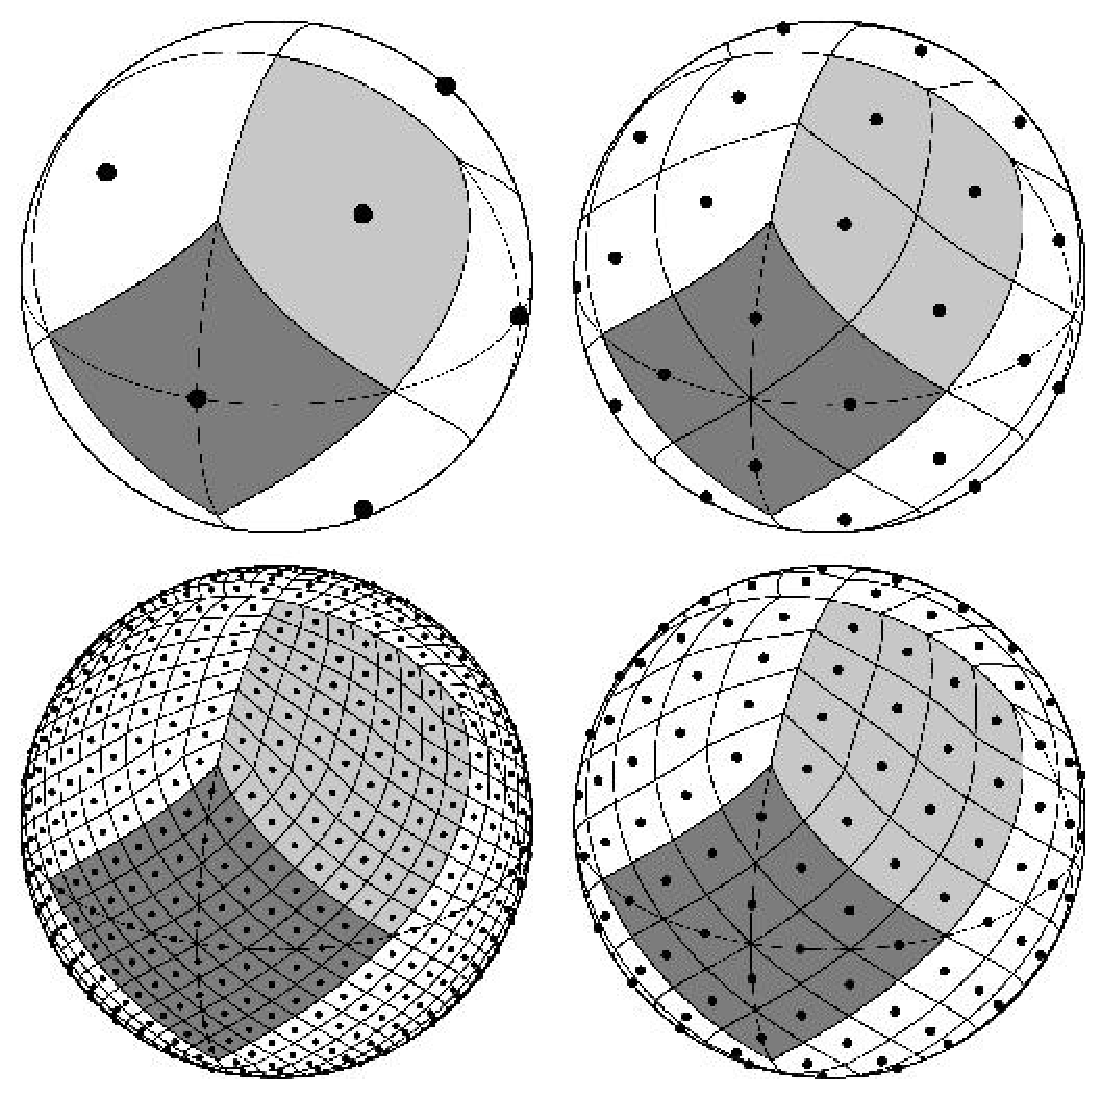
\includegraphics[width=0.6\linewidth]{healpix}}
\label{img:healpix}
\end{figure}

\end{frame}	

\subsection{Распределение разностей паралаксов}\label{sub:smthhealpix}
\begin{frame}[<alignment>]
\frametitle{Распределение разностей паралаксов}

\end{frame}	

\subsection{Сферические функции}\label{sistem}  
\begin{frame}[<alignment>]
\frametitle{Сферические функци}

\end{frame}	

\subsection{Сферические гармоники}\label{sistem}  
\begin{frame}[<alignment>]
\frametitle{Сферические гармоники}
d;e[

\end{frame}	

\section{Заключение}\label{conclusion}
\begin{frame}[<alignment>]
\frametitle{Заключение}
Звезды по HIP ближе на $6\%$.

Мы получили очень важные и нужные результаты. в виде разложения на гармоники.\\

Спасибо за внимание!
\end{frame}	


%\setcounter{framenumber}{0} %or \setcounter{framenumber}{1}

%\setcounter{framenumber}{\value{finalframe}}
\appendix
\newcounter{finalframe}
\setcounter{finalframe}{\value{framenumber}}
\begin{frame}

\frametitle{Инструменты которыми, пользовались в исследования}
\begin{figure}[H]
\begin{minipage}[h]{0.13\linewidth}
\center{\includegraphics[width=0.7\linewidth]{c_logo}} 
\end{minipage}
\hfill
\begin{minipage}[h]{0.13\linewidth}
\center{\includegraphics[width=.5\linewidth]{ISO_C++_Logo}} 
\end{minipage}
\hfill
\begin{minipage}[h]{0.23\linewidth}
\center{\includegraphics[width=.7\linewidth]{fortran}} 
\end{minipage}
\hfill
\begin{minipage}[h]{0.23\linewidth}
\center{\includegraphics[width=.5\linewidth]{python}} 
\end{minipage}

\vfill
\begin{minipage}[h]{0.31\linewidth}
\center{\includegraphics[width=0.7\linewidth]{IPy_header}} 
\end{minipage}
\hfill
\begin{minipage}[h]{0.31\linewidth}
\center{\includegraphics[width=.5\linewidth]{jupyter_logo}} 
\end{minipage}
\hfill
\begin{minipage}[h]{0.31\linewidth}
\center{\includegraphics[width=.5\linewidth]{Anaconda_Logo}} 
\end{minipage}

\vfill
\begin{minipage}[h]{0.31\linewidth}
\center{\includegraphics[width=0.5\linewidth]{numpy_logo}} 
\end{minipage}
\hfill
\begin{minipage}[h]{0.31\linewidth}
\center{\includegraphics[width=.85\linewidth]{pandas_logo}} 
\end{minipage}
\hfill
\begin{minipage}[h]{0.31\linewidth}
\center{\includegraphics[width=.5\linewidth]{scipy}} 
\end{minipage}
\vfill

\begin{minipage}[h]{0.7\linewidth}
\center{\includegraphics[width=.5\linewidth]{nplotlib_logos2}} 
\end{minipage}
%\caption{инстуременты разработки}
%\label{ris:experimentalcorrelationsignals}
\end{figure}

\end{frame}

\section{Заsdfsdf}\label{codfnclusion}
\begin{frame}[<alignment>]
\frametitle{Заключениsdfsе}

sdfasdfasf
dsaf
adsf.


\end{frame}	


\section{Заsdfsdf}\label{codfnclusion}
\begin{frame}[<alignment>]
\frametitle{Заключениsdfsе}

sdfasdfasf
dsaf
adsf.


\end{frame}	



\setcounter{framenumber}{\value{finalframe}}
\end{document}